% Answer key for the transcribed ECON 5030 midterm (ECON5030_Midterm.tex): each question in full, solution underneath.
\documentclass[11pt]{article}
\usepackage[letterpaper,margin=1.15in,top=1.1in]{geometry}
\usepackage{amsmath,amssymb}
\usepackage[T1]{fontenc}
\usepackage{lmodern}
\usepackage{enumitem}
\usepackage{cmap}
\usepackage{tikz}
\usetikzlibrary{trees}

\pagestyle{myheadings}
\markright{ECON 5030 Midterm: Answer Key}

\newcommand{\bw}{\overline{\omega}}

\setlist[description]{leftmargin=2.2em,labelindent=0pt,labelwidth=2em,itemsep=0.6em,font=\normalfont\bfseries}

\newenvironment{solution}{\par\smallskip\noindent\textbf{Answer.} }{\par\medskip}

\tikzset{dec/.style={circle,fill,inner sep=1.5pt}}

% Two-stage game tree: #1,#2 = P1 actions; #3,#4 = P2 actions; #5-#8 = payoffs at
% (#1,#3), (#1,#4), (#2,#3), (#2,#4). Bold edges mark the backward-induction choices.
\newcommand{\gtree}[8]{%
\begin{center}
\begin{tikzpicture}[level distance=14mm, level 1/.style={sibling distance=52mm},
  level 2/.style={sibling distance=26mm}, every node/.style={font=\small}]
\node[dec,label=above:{P1}]{}
  child{node[dec,label=left:{P2}]{}
    child{node[below]{#5} edge from parent node[left]{$#3$}}
    child{node[below]{#6} edge from parent node[right]{$#4$}}
    edge from parent node[left]{$#1$}}
  child{node[dec,label=right:{P2}]{}
    child{node[below]{#7} edge from parent node[left]{$#3$}}
    child{node[below]{#8} edge from parent node[right]{$#4$}}
    edge from parent node[right]{$#2$}};
\end{tikzpicture}
\end{center}}

\title{Midterm Exam: Answer Key}
\author{Econ 511}
\date{}

\begin{document}
\maketitle
\thispagestyle{myheadings}

\section{Preferences}

\noindent Consider an agent with preferences over $X=[0,1]\times[0,1]$ defined as follows: For all $x,x'\in X$,
\begin{align*}
x &\succ x' \text{ if } x_1 > x_1' \text{ and } x_1+x_2 > x_1'+x_2',\\
x' &\succ x \text{ if } x_1 > x_1' \text{ and } x_1+x_2 > x_1'+x_2'\\
x &\succ x' \text{if } x_1 = x_1' \text{ and } x_2 < x_2'
\end{align*}

\begin{solution}
\emph{Reading the definition.} Read literally, lines 1 and 2 have the same condition, so they would give both $x\succ x'$ and $x'\succ x$. That is impossible for a strict preference, so the second line must be a typo for
\[
x'\succ x \text{ if } x_1>x_1' \text{ and } x_1+x_2 < x_1'+x_2'.
\]
Under this reading, for points with different first coordinates the bundle with the larger sum $x_1+x_2$ is strictly preferred. For points with the same first coordinate, the bundle with the \emph{smaller} $x_2$ is strictly preferred. Nothing is said when $x_1\neq x_1'$ and the sums are equal. (If you use the literal reading instead, say so: $\succ$ is then not even asymmetric, and every answer below is ``no''.)
\end{solution}

\begin{description}
\item[1.1] Write the definition of complete preferences clearly demonstrate that these preferences are (or are not) complete on $X$.
\begin{solution}
\emph{Definition.} $\succsim$ is complete on $X$ if for all $x,x'\in X$, $x\succsim x'$ or $x'\succsim x$ (or both).

\emph{Not complete.} Take $x=(0.6,0.2)$ and $x'=(0.4,0.4)$. Then $x_1>x_1'$ but $x_1+x_2=0.8=x_1'+x_2'$. None of the three lines applies, so neither $x\succ x'$ nor $x'\succ x$ holds, and indifference is never defined between distinct bundles. The two bundles cannot be compared. The same happens for any pair with $x_1\neq x_1'$ on the same line $x_1+x_2=c$.
\end{solution}

\item[1.2] Write the definition of transitive preferences clearly demonstrate are (or are not) transitive on $X=\mathbb{R}^2$.
\begin{solution}
\emph{Definition.} $\succsim$ is transitive if for all $x,y,z$, $x\succsim y$ and $y\succsim z$ imply $x\succsim z$. For the strict part: $x\succ y$ and $y\succ z$ imply $x\succ z$.

\emph{Not transitive.} The third line ranks a \emph{smaller} sum higher when $x_1$ is tied, but the other lines rank a \emph{larger} sum higher when $x_1$ differs. This produces a cycle. Take
\[
a=(0.5,\,0.5),\qquad b=(0.5,\,0.6),\qquad c=(0.4,\,0.65).
\]
\begin{itemize}[itemsep=0pt]
\item $a\succ b$: $a_1=b_1$ and $a_2=0.5<0.6=b_2$ (line 3).
\item $b\succ c$: $b_1>c_1$ and $b_1+b_2=1.1>1.05=c_1+c_2$ (line 1).
\item $c\succ a$: $a_1>c_1$ but $a_1+a_2=1<1.05=c_1+c_2$ (line 2).
\end{itemize}
So $a\succ b\succ c\succ a$. Transitivity would require $a\succ c$, which contradicts $c\succ a$. These points lie in $[0,1]^2\subset\mathbb{R}^2$, so the preferences fail transitivity on $\mathbb{R}^2$ as well.
\end{solution}

\item[1.3] Does a utility function exist that represents these preferences on $X$. Explain.
\begin{solution}
No. If $u$ represents $\succsim$, then $x\succsim x'\iff u(x)\ge u(x')$, and $\succsim$ inherits the properties of $\ge$ on $\mathbb{R}$. Real numbers can always be compared, so $\succsim$ would be complete. Also, $\ge$ is transitive, so $\succsim$ would be transitive. These preferences fail both tests (1.1 and 1.2), so no utility function represents them. The cycle alone is enough: it would need $u(a)>u(b)>u(c)>u(a)$.
\end{solution}
\end{description}

\section{Game Theory}
\subsection{Timing and Strategies}

\noindent Take a simple two player game with each player having two actions. Player 1's set of actions is $\{a_1,b_1\}$. Player 2's set of actions is $\{c_2,d_2\}$. The players' payoffs over the four possible action combinations are as follows:
\begin{align*}
u_1(a_1,c_2) &= 45 & u_2(a_1,c_2) &= 50\\
u_1(a_1,d_2) &= 20 & u_2(a_1,d_2) &= 45\\
u_1(b_1,c_2) &= 50 & u_2(b_1,c_2) &= 15\\
u_1(b_1,d_2) &= 25 & u_2(b_1,d_2) &= 25
\end{align*}
Suppose this is a sequential choice game in which player 1 goes first, then player 2 observes player 1's choice and makes her choice.

\begin{description}
\item[2.1] Write the Normal Form of the game.
\begin{solution}
$\Gamma_N=\big[I,\{S_i\},\{u_i\}\big]$, where:
\begin{itemize}[itemsep=0pt]
\item $I=\{1,2\}$.
\item $S_1=\{a_1,b_1\}$.
\item Player 2 moves after seeing player 1's action, so her strategy is a complete contingent plan, one action for each of player 1's actions: $S_2=\{cc,\,cd,\,dc,\,dd\}$. Here $xy$ means ``play $x_2$ after $a_1$, play $y_2$ after $b_1$''.
\item $u_i(s_1,s_2)$ is the payoff of the outcome that the strategy profile $(s_1,s_2)$ produces (matrix in 2.2).
\end{itemize}
\end{solution}

\item[2.2] Construct the Game matrix.
\begin{solution}
Payoffs are $(u_1,u_2)$.
\begin{center}
\begin{tabular}{c|cccc}
 & $cc$ & $cd$ & $dc$ & $dd$\\ \hline
$a_1$ & $45,50$ & $45,50$ & $20,45$ & $20,45$\\
$b_1$ & $50,15$ & $25,25$ & $50,15$ & $25,25$
\end{tabular}
\end{center}
\end{solution}

\item[2.3] Find the set of strategies the remain after iterated deletion of strictly dominated strategies.
\begin{solution}
\emph{Player 2.} $cd$ strictly dominates $dc$: $50>45$ against $a_1$ and $25>15$ against $b_1$. Delete $dc$. The other comparisons give only weak dominance or none. $cd$ weakly dominates $cc$ ($50=50$, $25>15$) and $dd$ ($50>45$, $25=25$), but weak dominance does not count here. $cc$ and $dd$ do not dominate each other.

\emph{Player 1.} Against $cc,cd,dd$, $a_1$ gives $(45,45,20)$ and $b_1$ gives $(50,25,25)$. Neither dominates. Nothing else can be deleted.

\[
\text{Remaining: } S_1=\{a_1,b_1\},\qquad S_2=\{cc,\,cd,\,dd\}.
\]
\end{solution}

\item[2.4] Find the set of Nash Equilibrium.
\begin{solution}
Best responses:
\begin{itemize}[itemsep=0pt]
\item Player 1: $BR_1(cc)=b_1$, $BR_1(cd)=a_1$, $BR_1(dc)=b_1$, $BR_1(dd)=b_1$.
\item Player 2: $BR_2(a_1)=\{cc,cd\}$ (both 50), $BR_2(b_1)=\{cd,dd\}$ (both 25).
\end{itemize}
A cell is a NE when both players are best responding:
\[
NE=\{(a_1,cd),\ (b_1,dd)\}\qquad\text{with payoffs }(45,50)\text{ and }(25,25).
\]
\emph{Mixed equilibria (if you go further).} Player 2 can mix between strategies that tie, as long as player 1 still wants to stay.
\begin{itemize}[itemsep=0pt]
\item $a_1$ with $q\,cc+(1-q)\,cd$ is a NE for $q\le 0.8$. Player 1 gets 45 from $a_1$ and $25+25q$ from $b_1$.
\item $b_1$ with $r\,cd+(1-r)\,dd$ is a NE for $r\le 0.2$. Player 1 gets 25 from $b_1$ and $20+25r$ from $a_1$.
\end{itemize}
\end{solution}

\item[2.5] Write the Game Tree and find the set of Subgame prefect equilibrium.
\begin{solution}
\gtree{a_1}{b_1}{c_2}{d_2}{$(45,50)$}{$(20,45)$}{$(50,15)$}{$(25,25)$}
Backward induction:
\begin{itemize}[itemsep=0pt]
\item After $a_1$, player 2 picks $c_2$ ($50>45$). After $b_1$, she picks $d_2$ ($25>15$). So player 2 plays $cd$.
\item Player 1 anticipates this: $a_1\to 45$ and $b_1\to 25$, so she plays $a_1$.
\end{itemize}
\[
SPE=\{(a_1,\,cd)\},\qquad\text{outcome }(a_1,c_2)\text{ with payoffs }(45,50).
\]
The other NE $(b_1,dd)$ is not subgame perfect. It relies on the non-credible threat to play $d_2$ after $a_1$, which gives player 2 only 45 instead of 50.
\end{solution}
\end{description}

\subsection{Games with Different Preferences}

\noindent There are two players and each player $i$ has two actions $\{R_i,Q_i\}$. The money each player $i$ receives for the different action pairs is (in a game with player $j$) is described in the matrix below (\emph{this is not the Game Matrix}):
\[
\begin{array}{ccc@{\qquad}c}
 & & \multicolumn{2}{c}{P2}\\
 & & R_2 & Q_2\\
P1 & R_1 & \$9,\$9 & \$0,\$20\\
 & Q_1 & \$20,\$0 & \$2,\$2
\end{array}
\]

The game is sequential. Player 1 picks her action first and then player 2 observes the action of player 1 and player 2 picks his action. We will consider 3 cases of this game.

\emph{Case 1}: Both players only care about their own money with more money being strictly better than less.

\begin{description}
\item[2.6] Create a normal form for this game. Write the game matrix and find the set of Nash Equilibrium. Draw the game tree and find the set of Subgame perfect equilibrium.
\begin{solution}
\emph{Normal form.} $I=\{1,2\}$ and $S_1=\{R_1,Q_1\}$. Player 2 has strategies $S_2=\{RR,RQ,QR,QQ\}$, where $xy$ means: play $x_2$ after $R_1$ and $y_2$ after $Q_1$. Payoffs $u_i$ are each player's own money. Any increasing function of money works, so we use the dollar amounts.
\begin{center}
\begin{tabular}{c|cccc}
 & $RR$ & $RQ$ & $QR$ & $QQ$\\ \hline
$R_1$ & $9,9$ & $9,9$ & $0,20$ & $0,20$\\
$Q_1$ & $20,0$ & $2,2$ & $20,0$ & $2,2$
\end{tabular}
\end{center}
\emph{NE.} Best responses:
\begin{itemize}[itemsep=0pt]
\item Player 1: $BR_1(RR)=Q_1$, $BR_1(RQ)=R_1$, $BR_1(QR)=Q_1$, $BR_1(QQ)=Q_1$.
\item Player 2: $BR_2(R_1)=\{QR,QQ\}$, $BR_2(Q_1)=\{RQ,QQ\}$.
\end{itemize}
The only cell where both are best responding is
\[
NE=\{(Q_1,\,QQ)\},\qquad\text{payoffs }(\$2,\$2).
\]
\emph{SPE.}
\gtree{R_1}{Q_1}{R_2}{Q_2}{$(9,9)$}{$(0,20)$}{$(20,0)$}{$(2,2)$}
Backward induction:
\begin{itemize}[itemsep=0pt]
\item After $R_1$, player 2 picks $Q_2$ ($20>9$). After $Q_1$, he picks $Q_2$ ($2>0$).
\item Player 1 compares $R_1\to 0$ with $Q_1\to 2$ and picks $Q_1$.
\end{itemize}
\[
SPE=\{(Q_1,\,QQ)\},\qquad\text{outcome }(\$2,\$2).
\]
This is a sequential Prisoners' Dilemma. Both would prefer $(R_1,R_2)$ with $(\$9,\$9)$. Player 2 cannot commit to reciprocate $R_1$, so player 1 never plays it.
\end{solution}
\end{description}

\emph{Case 2}: Both players care about each other in a particular way. Each player only cares about the sum of the two players' money and strictly prefers more total money to less.

\begin{description}
\item[2.7] Create a normal form for this game. Write the game matrix and find the set of Nash Equilibrium. Draw the game tree and find the set of Subgame perfect equilibrium.
\begin{solution}
\emph{Normal form.} The players and strategy sets are the same as in 2.6. Now $u_1=u_2=$ total money:
\[
(R_1,R_2)\to 18,\quad (R_1,Q_2)\to 20,\quad (Q_1,R_2)\to 20,\quad (Q_1,Q_2)\to 4.
\]
\begin{center}
\begin{tabular}{c|cccc}
 & $RR$ & $RQ$ & $QR$ & $QQ$\\ \hline
$R_1$ & $18,18$ & $18,18$ & $20,20$ & $20,20$\\
$Q_1$ & $20,20$ & $4,4$ & $20,20$ & $4,4$
\end{tabular}
\end{center}
\emph{NE.} Best responses:
\begin{itemize}[itemsep=0pt]
\item Player 1: $BR_1(RR)=Q_1$, $BR_1(RQ)=R_1$, $BR_1(QR)=\{R_1,Q_1\}$, $BR_1(QQ)=R_1$.
\item Player 2: $BR_2(R_1)=\{QR,QQ\}$, $BR_2(Q_1)=\{RR,QR\}$.
\end{itemize}
\[
NE=\{(R_1,QR),\ (R_1,QQ),\ (Q_1,RR),\ (Q_1,QR)\}.
\]
Every NE gives total money \$20 and utility $(20,20)$.

\emph{SPE.}
\gtree{R_1}{Q_1}{R_2}{Q_2}{$(18,18)$}{$(20,20)$}{$(20,20)$}{$(4,4)$}
Backward induction:
\begin{itemize}[itemsep=0pt]
\item After $R_1$, player 2 picks $Q_2$ ($20>18$). After $Q_1$, he picks $R_2$ ($20>4$). So player 2 plays $QR$.
\item Player 1 then gets 20 from either action, so she is indifferent.
\end{itemize}
\[
SPE=\{(R_1,\,QR),\ (Q_1,\,QR)\}
\]
Player 1 may also mix between $R_1$ and $Q_1$ against $QR$. The outcomes are $(R_1,Q_2)$ with money $(\$0,\$20)$ or $(Q_1,R_2)$ with $(\$20,\$0)$, and utility $(20,20)$ either way. $(R_1,QQ)$ and $(Q_1,RR)$ are NE but not SPE, because each uses a non-optimal choice off the equilibrium path. Caring about the total removes the dilemma but creates multiple equilibria.
\end{solution}
\end{description}

\emph{Case 3}: There are 3 players: Player 1, Player 2a and Player 2b. Player 1 only cares about the sum of money of herself and Player 2b, with more money being strictly better. Player 2a only cares about her own money, with more money strictly better. Player 2b only cares about the sum of money of herself and Player 1, with more money being strictly better.

In this case, Player 1 makes her decision without knowing for sure who she is playing. With probability $\mu\in(0,1)$ she will play against Player 2a and with probability $1-\mu$ she will play against Player 2b. The player not playing the game (2a or 2b) gets zero money no matter what happens.

\begin{description}
\item[2.8] You will need to be a little creative to analyze this game. Create a game tree for this game and use a form of backward induction as your solution concept. Explain clearly the difficulties you faced in finding a way to analyze the game.
\begin{solution}
\emph{Utilities.} Write money as $(m_1,m_{2a},m_{2b})$. Then
\[
u_1=m_1+m_{2b},\qquad u_{2a}=m_{2a},\qquad u_{2b}=m_1+m_{2b}.
\]
Only increasing transformations of these matter for the analysis below.

\emph{Game tree.} Nature moves first and picks the opponent. Player 1 cannot see Nature's move, so her two nodes form one information set (dashed). The opponent then sees player 1's action. Leaves show $(u_1,\,u_{\text{opponent}})$. The idle player always gets 0.
\begin{center}
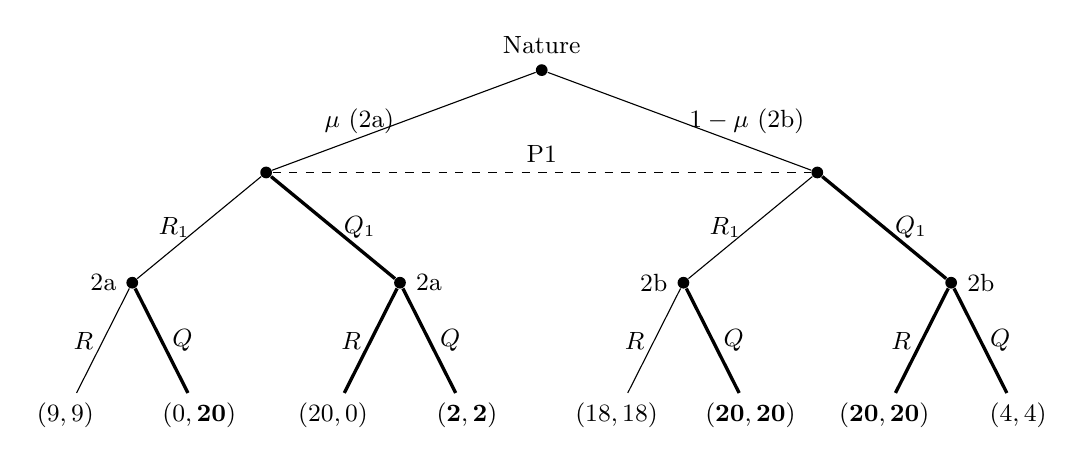
\begin{tikzpicture}[every node/.style={font=\small},
  level 1/.style={sibling distance=70mm, level distance=13mm},
  level 2/.style={sibling distance=34mm, level distance=14mm},
  level 3/.style={sibling distance=17mm, level distance=14mm}]
\node[dec,label=above:{Nature}]{}
  child{node[dec](L){}
    child{node[dec,label=left:{2a}]{}
      child{node[below]{$(9,9)$} edge from parent node[left]{$R$}}
      child{node[below]{$(0,\mathbf{20})$} edge from parent[very thick] node[right]{$Q$}}
      edge from parent node[left]{$R_1$}}
    child{node[dec,label=right:{2a}]{}
      child{node[below]{$(20,0)$} edge from parent node[left]{$R$}}
      child{node[below]{$(\mathbf{2},\mathbf{2})$} edge from parent[very thick] node[right]{$Q$}}
      edge from parent[very thick] node[right]{$Q_1$}}
    edge from parent node[left]{$\mu$\ (2a)}}
  child{node[dec](R){}
    child{node[dec,label=left:{2b}]{}
      child{node[below]{$(18,18)$} edge from parent node[left]{$R$}}
      child{node[below]{$(\mathbf{20},\mathbf{20})$} edge from parent[very thick] node[right]{$Q$}}
      edge from parent node[left]{$R_1$}}
    child{node[dec,label=right:{2b}]{}
      child{node[below]{$(\mathbf{20},\mathbf{20})$} edge from parent[very thick] node[left]{$R$}}
      child{node[below]{$(4,4)$} edge from parent node[right]{$Q$}}
      edge from parent[very thick] node[right]{$Q_1$}}
    edge from parent node[right]{$1-\mu$\ (2b)}};
\draw[dashed] (L)--(R) node[midway,above]{P1};
\end{tikzpicture}
\end{center}

\emph{Step 1: the second movers.} Each of their nodes starts a proper subgame, so ordinary backward induction applies.
\begin{itemize}[itemsep=0pt]
\item Player 2a (own money): after $R_1$ plays $Q$ ($20>9$). After $Q_1$ plays $Q$ ($2>0$).
\item Player 2b (sum with P1): after $R_1$ plays $Q$ ($20>18$). After $Q_1$ plays $R$ ($20>4$).
\end{itemize}

\emph{Step 2: player 1 at her information set.} She cannot condition on the opponent's type, so she compares the lotteries her two actions induce. In utility units, given the second movers' choices:
\begin{align*}
R_1:&\quad \text{vs.\ 2a: } 0+0=0, &&\text{vs.\ 2b: } 0+20=20,\\
Q_1:&\quad \text{vs.\ 2a: } 2+0=2, &&\text{vs.\ 2b: } 20+0=20.
\end{align*}
$Q_1$ is weakly better state by state, and strictly better against 2a. Since $\mu>0$, player 1 strictly prefers $Q_1$ for \emph{every} increasing vNM utility over the sum. With risk-neutral (linear) utility,
\[
EU(R_1)=20(1-\mu)\;<\;EU(Q_1)=2\mu+20(1-\mu)=20-18\mu.
\]
The gap is $2\mu>0$.

\emph{Solution.} Player 1 plays $Q_1$. 2a plays $Q$ after $R_1$ and $Q$ after $Q_1$. 2b plays $Q$ after $R_1$ and $R$ after $Q_1$. This holds for all $\mu\in(0,1)$. The realized money is $(\$2,\$2)$ against 2a and $(\$20,\$0)$ against 2b.

\emph{Difficulties.}
\begin{enumerate}[itemsep=0pt]
\item \emph{Three players, two possible games.} Only two of them actually play, and the idle one still needs a payoff (0). Player 1's utility depends on who she faces: 2b's money counts for her, 2a's does not. So the same money outcome means different utilities on the two sides of the tree.
\item \emph{Incomplete information.} Player 1's two decision nodes lie in one information set. No subgame starts there, so plain backward induction stops at that point. We add a chance move by Nature and require player 1 to choose one action for the whole information set, using her beliefs $(\mu,1-\mu)$.
\item \emph{Expected utility is needed.} Comparing actions means ranking lotteries, so we need vNM preferences. The problem only gives ordinal information (``more is better''), which is not enough in general. Here that problem disappears, because $Q_1$ is weakly better in each state. In general the answer could depend on $\mu$ and on risk attitudes.
\item \emph{Conflicting preferences with the same action names.} 2a and 2b respond differently to $Q_1$. Player 1 is effectively choosing against a mixture of a selfish and an altruistic opponent. This is a Bayesian game, and the solution is the extensive-form analogue of a Bayesian (perfect) equilibrium.
\end{enumerate}
\end{solution}
\end{description}

\section{Conceptual Questions}

\begin{description}
\item[3.1] Explain clearly the idea of the Independence Axiom. Why is this the exact assumption needed for the an expected utility form representation of preferences over lotteries?
\begin{solution}
\emph{Independence Axiom.} For all lotteries $L,L',L''$ and $\alpha\in(0,1)$:
\[
L\succsim L' \iff \alpha L+(1-\alpha)L''\ \succsim\ \alpha L'+(1-\alpha)L''.
\]
If you mix two lotteries with the same third lottery, their ranking does not change. The common part $L''$ happens in exactly the same states under both options, so it should not affect the comparison. Only the part that differs matters.

\emph{Why it is exactly what EU needs.} An expected utility form is $U(L)=\sum_n p_n u_n$. It is \emph{linear in probabilities}: $U(\alpha L+(1-\alpha)L'')=\alpha U(L)+(1-\alpha)U(L'')$.
\begin{itemize}[itemsep=0pt]
\item \emph{Necessary.} If $U$ is linear, mixing both lotteries with $L''$ adds the same $(1-\alpha)U(L'')$ to both sides and scales the rest by $\alpha>0$. So the ranking is preserved, and independence must hold.
\item \emph{Sufficient.} Conversely, independence makes indifference curves in the probability simplex straight lines that are parallel to each other. Together with completeness, transitivity and continuity, this is exactly the vNM theorem: the preferences have an EU representation, unique up to positive affine transformations.
\end{itemize}
Completeness, transitivity and continuity alone give some continuous utility over lotteries. Independence is the extra assumption that makes that utility linear in probabilities, which is what ``expected utility form'' means.
\end{solution}

\item[3.2] Define the Normal Form of a game. What are the two types of solution concepts we discussed in class for the Normal Form? Explain.
\begin{solution}
\emph{Normal form.} $\Gamma_N=\big[I,\{S_i\}_{i\in I},\{u_i(\cdot)\}_{i\in I}\big]$:
\begin{itemize}[itemsep=0pt]
\item a set of players $I$;
\item for each player a strategy set $S_i$, where each strategy is a complete contingent plan;
\item payoff functions $u_i:S_1\times\cdots\times S_I\to\mathbb{R}$ giving each player's vNM utility for every strategy profile.
\end{itemize}
Players are modeled as choosing their strategies simultaneously.

\emph{The two solution concepts.}
\begin{enumerate}[itemsep=0pt]
\item \emph{Dominance (iterated deletion of strictly dominated strategies; rationalizability).} A rational player never plays a strictly dominated strategy. Under common knowledge of rationality, everyone knows this, so dominated strategies can be deleted repeatedly. This uses only rationality and common knowledge of it, with no assumption that beliefs are correct. It often leaves many strategies (2.3 deletes only one).
\item \emph{Nash equilibrium.} A profile $s^*$ such that $u_i(s_i^*,s_{-i}^*)\ge u_i(s_i,s_{-i}^*)$ for all $s_i$ and all $i$. Every player best-responds to the others' actual strategies. This adds the assumption that beliefs are correct (mutually consistent). It is sharper, but it can include non-credible threats in dynamic games. That is why we refine it to SPE (2.5).
\end{enumerate}
\end{solution}

\item[3.3] Lets suppose you wanted to apply game theory to better understand a military conflict (like the current conflict in the middle east). What are the difficulties for the application of game theoretic reasoning to understand such a scenario?
\begin{solution}
Any well-argued set of points earns credit. Strong answers tie each difficulty to a part of the model:
\begin{itemize}[itemsep=0pt]
\item \emph{Players.} Who are they? States, governments, militaries, factions, non-state groups, allies and outside powers. Each is a coalition, not a single decision maker with coherent preferences.
\item \emph{Payoffs.} Preferences are unknown and not just money. They include ideology, survival, domestic politics, reputation and concern for others' outcomes (as in Cases 2 and 3). Misjudging preferences changes the predicted equilibrium completely (compare 2.6 with 2.7).
\item \emph{Information.} It is incomplete and asymmetric. Players are unsure about opponents' types, capabilities and intentions (like player 1 in Case 3). This calls for beliefs, Bayesian updating, signaling and bluffing.
\item \emph{Strategies and timing.} Action sets are huge and partly continuous, the order of moves is unclear, and the interaction is repeated and dynamic. Writing a complete game tree or normal form is not realistic.
\item \emph{Credibility and commitment.} Threats and promises may not be credible (SPE vs.\ NE), and there are few enforcement mechanisms.
\item \emph{Equilibrium selection and rationality.} There can be multiple equilibria (2.7). The assumptions of common knowledge of rationality and correct beliefs are strong in high-stakes, emotional situations. Outcomes are hard to observe, so the model is hard to test.
\end{itemize}
\end{solution}

\item[3.4] At this point in time, what is the most valuable new insight you learned from this course? (Anything reasonable gets you points. You can define ``valuable'' anyway you like)
\begin{solution}
Any reasonable, explained answer gets full credit. \emph{Sample answer:} the gap between Nash and subgame perfect equilibrium. An outcome can look stable when each player's strategy is a best response, yet it can rely on a threat that would never be carried out (as $(b_1,dd)$ in 2.4). Asking ``would this player actually do that when the time comes?'' is a useful test for strategic situations in general, from negotiations to policy.
\end{solution}
\end{description}

\section{General Equilibrium Model of Exchange Economy}

\noindent Consider two consumers with preferences on $X=\mathbb{R}^2_+$. The two consumers' preferences are represented by the utility functions:
\begin{align*}
u^1(x_1^1,x_2^1) &= \left(x_1^1\right)^{1/8}\left(x_2^1\right)^{7/8}\\
u^2(x_1^2,x_2^2) &= \left(x_1^2\right)^{7/8}\left(x_2^2\right)^{1/8}
\end{align*}
Assume that prices are strictly positive $p=(p_1,p_2)\gg 0$. For now consider each consumer to have a wealth $w^i>0$.

\begin{description}
\item[4.1] Make a clear argument why we only need to consider the case that the budget constraint holds with equality (Walras' Law).
\begin{solution}
Both utilities are strictly increasing in each good on $\mathbb{R}^2_{++}$, so preferences are monotone and hence \emph{locally nonsatiated}. Suppose an optimal bundle $x^*$ had $p\cdot x^*<w^i$. Then there is room to buy a little more of both goods, $x^*+(\varepsilon,\varepsilon)$, and it is still affordable for small $\varepsilon>0$. It is strictly better, which contradicts optimality. Any bundle with a zero component gives $u=0$, while spending $w^i$ on both goods gives $u>0$, so the optimum is interior. Therefore $p\cdot x^*=w^i$ and we can solve with an equality constraint.
\end{solution}

\item[4.2] Write the Lagrangian for the two consumers' UMAX problems
\begin{solution}
\begin{align*}
\mathcal{L}^1&=\left(x_1^1\right)^{1/8}\left(x_2^1\right)^{7/8}+\lambda^1\big(w^1-p_1x_1^1-p_2x_2^1\big),\\
\mathcal{L}^2&=\left(x_1^2\right)^{7/8}\left(x_2^2\right)^{1/8}+\lambda^2\big(w^2-p_1x_1^2-p_2x_2^2\big).
\end{align*}
Using the monotone transformation $\ln u$ is equivalent and easier, for example $\tfrac18\ln x_1^1+\tfrac78\ln x_2^1+\lambda^1(w^1-p\cdot x^1)$.
\end{solution}

\item[4.3] Write the first order conditions (FOCs) and second order conditions (SOCs). Explain what the SOCs tell us about the solution to the problem.
\begin{solution}
\emph{FOCs} (consumer 1; consumer 2 swaps $\tfrac18\leftrightarrow\tfrac78$):
\[
\frac{1}{8}\frac{u^1}{x_1^1}=\lambda^1 p_1,\qquad \frac{7}{8}\frac{u^1}{x_2^1}=\lambda^1 p_2,\qquad p_1x_1^1+p_2x_2^1=w^1.
\]
Dividing the first two gives $MRS=\dfrac{x_2^1}{7x_1^1}=\dfrac{p_1}{p_2}$. For consumer 2: $\dfrac{7x_2^2}{x_1^2}=\dfrac{p_1}{p_2}$.

\emph{SOC.} With one constraint and two goods, a maximum requires the bordered Hessian to have a positive determinant at the critical point:
\[
\bar H=\begin{pmatrix}0&p_1&p_2\\ p_1&u_{11}&u_{12}\\ p_2&u_{12}&u_{22}\end{pmatrix},\qquad
|\bar H|=2p_1p_2u_{12}-p_2^2u_{11}-p_1^2u_{22}>0.
\]
For Cobb--Douglas, $u_{11}<0$, $u_{22}<0$ and $u_{12}>0$, so every term is positive and the condition holds.

\emph{Meaning.} The utility is quasi-concave (here in fact concave, since the exponents sum to 1) and the budget set is convex. So the critical point is a \emph{maximum}, it is the \emph{global} maximum, and it is \emph{unique}. The FOCs therefore pin down the demand functions.
\end{solution}

\item[4.4] Solve for the demand functions for both consumers.
\begin{solution}
Cobb--Douglas consumers spend a fixed share of wealth on each good.
\[
x^1(p,w^1)=\left(\frac{w^1}{8p_1},\ \frac{7w^1}{8p_2}\right),\qquad
x^2(p,w^2)=\left(\frac{7w^2}{8p_1},\ \frac{w^2}{8p_2}\right).
\]
For consumer 1: from the MRS, $p_2x_2^1=7p_1x_1^1$. Substituting into the budget gives $8p_1x_1^1=w^1$. Consumer 2 is symmetric.
\end{solution}
\end{description}

Consider a market with these two consumer and two goods that is perfectly competitive. There is total endowment of each good in the economy is $\bw_1$ and $\bw_2$. Consumer 1's wealth is based on the the endowments $w^1=\lambda\bw_1+(1-\lambda)\bw_2$ and $w^2=(1-\lambda)\bw_1+\lambda\bw_2$, where the parameter $\lambda\in[0,1]$ and the total endowment of each good in the economy is $(\bw_1,\bw_2)$.

\begin{solution}
\emph{Reading the setup.} Wealth comes from selling endowments at market prices. Consumer 1 owns $e^1=(\lambda\bw_1,(1-\lambda)\bw_2)$ and consumer 2 owns $e^2=((1-\lambda)\bw_1,\lambda\bw_2)$, so
\[
w^1=p_1\lambda\bw_1+p_2(1-\lambda)\bw_2,\qquad w^2=p_1(1-\lambda)\bw_1+p_2\lambda\bw_2.
\]
The printed formulas leave out the prices. If wealth were a fixed number, prices would not need normalizing, which contradicts 4.6.
\end{solution}

\begin{description}
\item[4.5] Write the Market Clearing Conditions (MCCs) and explain what they mean.
\begin{solution}
\begin{align*}
\text{Good 1:}&\quad \frac{w^1}{8p_1}+\frac{7w^2}{8p_1}=\bw_1,\\
\text{Good 2:}&\quad \frac{7w^1}{8p_2}+\frac{w^2}{8p_2}=\bw_2.
\end{align*}
In each market, the total quantity the consumers demand at prices $p$ (given the wealth their endowments generate) equals the total amount available. There is no excess demand or supply, so each consumer's optimal plan can actually be carried out.
\end{solution}

\item[4.6] Explain why you must normalize a price to solve for the prices using the MCCs.
\begin{solution}
There are two reasons, and they amount to the same thing:
\begin{enumerate}[itemsep=0pt]
\item Demand is homogeneous of degree 0 in $p$. Wealth $w^i=p\cdot e^i$ scales with $p$, so $x^i(tp,tp\cdot e^i)=x^i(p,p\cdot e^i)$. If $p^*$ clears markets, so does $tp^*$ for every $t>0$. Only \emph{relative} prices are determined.
\item By Walras' Law, $p\cdot\big(\sum_i x^i-\bw\big)=0$ for every $p$. So if one market clears, the other does too. We have two equations but only one independent one, with two unknowns.
\end{enumerate}
Fixing a numeraire (e.g.\ $p_2=1$) removes the free scale and leaves one equation in one unknown.
\end{solution}

\item[4.7] Solve the MMCs for the vector $p^*$.
\begin{solution}
Normalize $p_2=1$ and write $p=p_1$. Good 1's MCC gives $w^1+7w^2=8p\bw_1$, where
\begin{align*}
w^1+7w^2&=p\bw_1\big[\lambda+7(1-\lambda)\big]+\bw_2\big[(1-\lambda)+7\lambda\big]\\
&=p\bw_1(7-6\lambda)+\bw_2(1+6\lambda).
\end{align*}
Setting this equal to $8p\bw_1$ gives $p\bw_1(1+6\lambda)=\bw_2(1+6\lambda)$. Since $1+6\lambda>0$,
\[
\boxed{\;p^*=\Big(\frac{\bw_2}{\bw_1},\ 1\Big),\qquad \frac{p_1^*}{p_2^*}=\frac{\bw_2}{\bw_1}.\;}
\]
\emph{Check (good 2).} $7w^1+w^2=p\bw_1(1+6\lambda)+\bw_2(7-6\lambda)=8\bw_2$ when $p\bw_1=\bw_2$. \checkmark

At $p^*$, both wealths equal $w^1=w^2=\bw_2$. The allocation is $x^{1*}=\big(\tfrac{\bw_1}{8},\tfrac{7\bw_2}{8}\big)$ and $x^{2*}=\big(\tfrac{7\bw_1}{8},\tfrac{\bw_2}{8}\big)$, which adds up to $(\bw_1,\bw_2)$.
\end{solution}

\item[4.8] Explain exactly how the prices change as the parameter $\lambda$ changes.
\begin{solution}
They do not change: $p_1^*/p_2^*=\bw_2/\bw_1$ for every $\lambda\in[0,1]$, because the factor $(1+6\lambda)$ cancels in 4.7. The reason is that at $p^*$ the economy's total supply of each good has the same value, $p_1^*\bw_1=p_2^*\bw_2$. Consumer $i$ owns a fraction $\lambda$ of one good and $1-\lambda$ of the other, so her wealth is $\lambda V+(1-\lambda)V=V$ whatever $\lambda$ is. Changing $\lambda$ reshuffles endowments without changing anyone's wealth at these prices. Demand is unchanged, so markets still clear at the same prices, and even the allocation does not depend on $\lambda$. (With equal wealth, aggregate spending on good 1 is $\tfrac12(\tfrac18+\tfrac78)=\tfrac12$ of total wealth, which confirms $p_1\bw_1=p_2\bw_2$.)
\end{solution}

\item[4.9] Explain exactly how the prices change as $(\bw_1,\bw_2)$. Give an intuition for this result.
\begin{solution}
$p_1^*/p_2^*=\bw_2/\bw_1$.
\begin{itemize}[itemsep=0pt]
\item Increasing $\bw_1$ lowers the relative price of good 1 in proportion: doubling $\bw_1$ halves $p_1/p_2$.
\item Increasing $\bw_2$ raises $p_1/p_2$ in proportion.
\item Scaling both endowments by the same factor leaves prices unchanged, since only relative scarcity matters.
\end{itemize}
\emph{Intuition.} Prices reflect scarcity. A good that becomes more plentiful must become relatively cheaper for consumers to be willing to absorb the extra units. With Cobb--Douglas preferences and equal wealth, the economy as a whole spends exactly half its wealth on each good, so the \emph{values} $p_1\bw_1$ and $p_2\bw_2$ must be equal. Expenditure shares are fixed, so the price elasticity is unitary: a 1\% rise in the supply of a good lowers its relative price by exactly 1\%.
\end{solution}
\end{description}

\end{document}
